\uuid{uITn}
\exo7id{4995}
\titre{exo7 4995}
\auteur{quercia}
\organisation{exo7}
\datecreate{2010-03-17}
\isIndication{false}
\isCorrection{true}
\chapitre{Courbes planes}
\sousChapitre{Courbes définies par une condition}

\contenu{
\texte{
Soit $\mathcal{C}$ une courbe du plan. A un point $M$ un point de $\mathcal{C}$, on associe les
points $T$ et $N$ selon le dessin :
$$
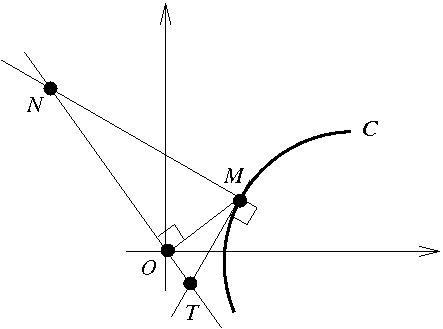
\includegraphics[height=4cm]{../images/img004995-1}
$$

Déterminer les courbes vérifiant la condition suivante :
}
\begin{enumerate}
    \item \question{$\overline{OT} = {}$cste.}
\reponse{$\rho = \frac1{a\theta+b}$.}
    \item \question{$\overline{ON} = {}$cste.}
\reponse{$\rho = a\theta+b$. (Spirale d'Archimède)}
\end{enumerate}
}
